% !TEX root = ../main.tex

%-- number of constraints?
\chapter{Proof construction}
We will be using Circom to generate an airthmetic circuit, and SnarkJS for the proof generation.

\paragraph{Circom} is a domain-specific language for creating arithmetic circuits, which are used in zk-SNARKs.
The circuit code can be written to specify the desired constraints.
Circom allows expressing the circuit's arithmetic operations, constraints, input and output in a concise and readable manner.
Once the circuit is designed, it needs to be compiled into a format suitable for zk-SNARKs.


\paragraph{SnarkJS} is a JavaScript library that provides tools for working with zk-SNARKs, including circuit compilation.
After compilation, SnarkJS facilitates generating zk-SNARK proofs for specific instances of the circuit.
SnarkJS also provides utilities for verifying the proofs.

\section{Proof of liabilities}
The proof of liabilities operates on a list of balances and a list of email hashes as private inputs.
The first purpose of the circuit is to validate that all values are non-negative and that all balances fall within a specified range. 
These verifications are crucial to prevent overflow or underflow issues, given that the operations occur within a finite field. 

Subsequently, the proof of liabilities constructs a Merkle tree and provides outputs the total balance sum and the root hash of the Merkle tree.

\paragraph{Inputs}
\begin{enumerate}

    \item List of balance (private)
    
    \item List of email hash (private)
    
    \end{enumerate}

\paragraph{Outputs}
\begin{enumerate}
    \item Balance Sum (public)
    \item Root hash (public)
    \item No negative values (private) - boolean
    \item All small range (private) - boolean
    \end{enumerate}

This proof of liabilities operates as intended because it returns the sum of the liabilities, which is exact because of the checks. 
It also returns the root hash, insuring you cannot alter any values insiside the merkle tree. The merkle tree is hidden so that we do not
give any information about users and their balances.
The root hash will be used to verify the inclusion of the balances.


In a complete proof of reserves, the balance sum would be a private output. We would have another circuit proving that the sum of liabilities is smaller
than the sum of assets, without revelaing the balance.


\section{Proof of inclusion} 
The proof of inclusion aims to prove that the balance of a user is included in the Merkle Tree created in the proof of liabilities.
To prove that a balance is included, it is sufficient to show that you know the Merkle path of a user balance,
which we define using the list of neighbors sum, hash and binary. 
The neighbors binary variable indicates whether the neighbor is on the left or the right. 
The root hash, root sum, user balance and user email hash are public because it needs to be shown which user is in which tree.

In the figure 4.1, Charlie is defined as the user. The merkle path is composed of the three blue nodes. In each blue nodes we can find the variables of the lists,
namely the binary (left or right), the sum and the hash.
\begin{figure}[H]
    \centering
    \includegraphics[width=130mm]{MerklePath.png}
    \caption{Merkle Path \cite{BM22}}
    \label{overflow}
    \end{figure}

\paragraph{Inputs}
\begin{enumerate}

    \item List of neighbors sum (private)
    
    \item List of neighbors hash (private)

    \item List of neighbors binary (private)

    \item Root hash (public)

    \item Root sum (public)

    \item User balance (public)

    \item User email hash (public)
    
    \end{enumerate}

\paragraph{Outputs}
\begin{enumerate}
    \item Balance included (public) - boolean
    \end{enumerate}

\paragraph{}
In the circuit, we verify that the combination of the user balance,sum and mekle path gives the right root hash and root sum. There is no additionnal
verifications since they are already done for this root hash, in the proof of liabilities.


\section{Daily proof of liabilities} 


\section{Daily proof of inclusion} 
Because a marketplace can have millions of users, it is impractical to build a proof of inclusion for every single user everyday. 
It is the user's responsibility to ask for a proof that its balance is included in the published Merkle tree.
 In an ideal world, a Merkle tree would be published at least daily, so it is once again impractical to require every user to verify their inclusion everyday. 
 Every user verifying its inclusion in the tree increases the chance that the proof of liabilities is valid and includes every single balance. 
 This is why it is primordial to find a way to make it easier to verify the inclusion. This is where Nova folding schemes come in.

The novel way to do proof of inclusion is to generate a proof of inclusion that is valid from the day of creation of the account, to the requested day by the user. 
Normally you would have to do 500 different proofs for 500 days. However, we saw in the previous section that the nova folding scheme allow you to fold the 500 proofs into 1 proof.
Verifying this one proof is the equivalent of verifying the 500, or any other number of days required. 

Previously, when requesting a proof of inclusion, the user would only have the proof that the latest published Merkle tree contains their balance. 
Now, it proves that the balance was contained in every Merkle tree published previously. 
It ensures that a bad entity would not be able to change who owns which balance throughout the days. 
%--description of the circuit
%--description of the necessity of having multiple verifiers

\begin{figure}[H]
    \centering
    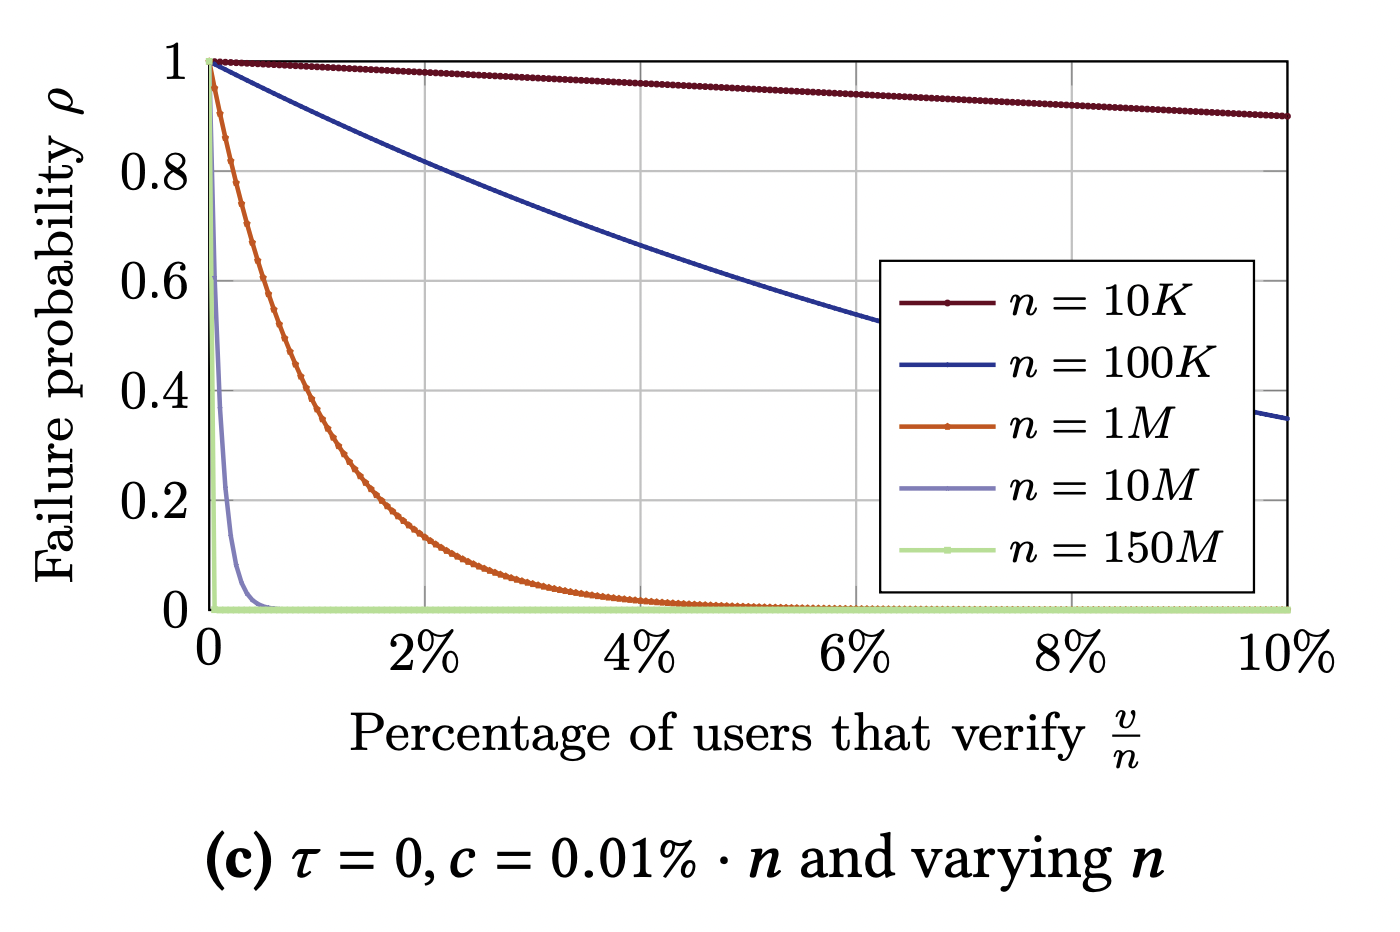
\includegraphics[width=130mm]{FailureProbability.png}
    \caption{Failure Probability \cite{GP21}}
    \label{overflow}
    \end{figure}

%Mina proof of recursion
%summa
%https://summa.gitbook.io/summa/v/1/circuits/merkle-sum-tree-inclusion